\documentclass[a4paper]{article}
\usepackage[T1]{fontenc}			% \chapter package
\usepackage[italian]{babel}
\usepackage[italian]{isodate}  		% date format
\usepackage{graphicx}				% manage images
\usepackage{amsfonts}
\usepackage{booktabs}				% high quality tables
\usepackage{amsmath}				% math package
\usepackage{amssymb}				% another math package (e.g. \nexists)
\usepackage{bm}                     % bold math symbols
\usepackage{mathtools}				% emphasize equations
\usepackage{stmaryrd} 				% '\llbracket' and '\rrbracket'
\usepackage{amsthm}					% better theorems
\usepackage{enumitem}				% manage list
\usepackage{pifont}					% nice itemize
\usepackage{cancel}					% cancel math equations
\usepackage{caption}				% custom caption
\usepackage[]{mdframed}				% box text
\usepackage{multirow}				% more lines in a table
\usepackage{textcomp, gensymb}		% degree symbol
\usepackage[x11names]{xcolor}		% RGB color
\usepackage[many]{tcolorbox}				% colorful box
\usepackage{multicol}				% more rows in a table (used for the lists)
\usepackage{listings}
\usepackage{url}
\usepackage{qrcode}
\usepackage{fontawesome5}
\usepackage{ragged2e}
\usepackage{cite}                   % references
\usepackage{imakeidx}               % index
\makeindex[program=makeindex, columns=2,
           title=Index, 
           intoc,
           options={-s index-style.ist}]


\definecolor{codegreen}{rgb}{0,0.6,0}
\definecolor{codegray}{rgb}{0.5,0.5,0.5}
\definecolor{codepurple}{rgb}{0.58,0,0.82}
\definecolor{backcolour}{rgb}{0.95,0.95,0.92}
\lstdefinestyle{mystyle}{
    backgroundcolor=\color{backcolour},   
    commentstyle=\color{codegreen},
    keywordstyle=\color{magenta},
    numberstyle=\tiny\color{codegray},
    stringstyle=\color{codepurple},
    basicstyle=\ttfamily\footnotesize,
    breakatwhitespace=false,         
    breaklines=true,                 
    captionpos=b,                    
    keepspaces=true,                 
    numbers=left,                    
    numbersep=5pt,                  
    showspaces=false,                
    showstringspaces=false,
    showtabs=false,                  
    tabsize=2
}
\lstset{style=mystyle}


% draw a frame around given text
\newcommand{\framedtext}[1]{%
	\par%
	\noindent\fbox{%
		\parbox{\dimexpr\linewidth-2\fboxsep-2\fboxrule}{#1}%
	}%
}


% table of content links
\usepackage{xcolor}
\usepackage[linkcolor=black, citecolor=blue, urlcolor=cyan]{hyperref} % hypertexnames=false
\hypersetup{
	colorlinks=true
}


\newtheorem{theorem}{\textcolor{Red3}{\underline{Theorem}}}
\renewcommand{\qedsymbol}{QED}
\newcommand{\dquotes}[1]{``#1''}
\newcommand{\longline}{\noindent\rule{\textwidth}{0.4pt}}
\newcommand{\circledtext}[1]{\raisebox{.5pt}{\textcircled{\raisebox{-.9pt}{#1}}}}
\newcommand{\definition}[1]{\textcolor{Red3}{\textbf{#1}}\index{#1}}
\newcommand{\example}[1]{\textcolor{Green4}{\textbf{#1}}}
\newcommand{\highspace}{\vspace{1.2em}\noindent}


\begin{document}
    \newcounter{definition}[section]
    \newcounter{example}[section]
    
    \newtcolorbox[use counter = definition]{definitionbox}{%
        colback=red!5!white,
        colframe=red!75!black,
        fonttitle=\bfseries,
        title=Definition \thetcbcounter %
    }
    
    \newtcolorbox[use counter = example]{examplebox}{%
        breakable,
        enhanced,
        colback=Green4!5!white,
        colframe=Green4!75!black,
        fonttitle=\bfseries,
        title=Example \thetcbcounter %
    }

    \author{260236}
	\title{Calcolo Numerico - Appunti}
	\date{\printdayoff\today}
	\maketitle

	\newpage

    \section*{Prefazione}

    Ogni sezione di teoria presente in questi appunti, è stata ricavata dalle seguenti risorse:
    \begin{itemize}
        \item Calcolo Scientifico: Esercizi e problemi risolti con MATLAB e Octave.\cite{quarteroni2017calcolo}
    \end{itemize}
    Altro:
    \begin{itemize}
        \item[\faIcon{github}] \href{https://github.com/AndreVale69/HPC-E-PoliMI-university-notes}{GitHub repository}
    \end{itemize}
    
    \newpage
	
	\tableofcontents

    \newpage

    \section{Equazioni non lineari}

    \subsection{Introduzione}

    Il \textbf{calcolo degli zeri di una funzione} $f$ reale di variabile reale o delle \textbf{radici dell'equazione} $f\left(x\right)=0$, è un problema assai ricorrente nel Calcolo Scientifico.

    \highspace
    In generale, \emph{non è possibile} approntare metodi numerici che calcolino gli zeri di una generica funzione in un numero finito di passi. I metodi numerici per la risoluzione di questo problema sono pertanto necessariamente \emph{iterativi}. A partire da uno o più dati iniziali, scelti convenientemente, essi generano una successione di valori $x^{\left(k\right)}$ che, sotto opportune ipotesi, convergerà ad uno zero $\alpha$ della funzione $f$ studiata.

    \longline

    \subsection{Il metodo di bisezione (o iterativo)}

    Sia $f$ una funzione continua in $\left[a,b\right]$ tale che $f\left(a\right)f\left(b\right) < 0$. Per cui, vale il \href{https://www.youmath.it/lezioni/analisi-matematica/limiti-continuita-e-asintoti/723-teorema-degli-zeri.html}{teorema degli zeri di una funzione continua}, ossia $f$ ammette almeno uno zero in $\left(a,b\right)$.

    \highspace
    Si supponga che ci sia un solo zero, indicato con $\alpha$ e nel caso in cui ce ne sia più di uno, individuare un intervallo tale che ne contenga solo uno.

    \highspace
    Il \definition{metodo di bisezione} (o \textbf{iterativo}\index{metodo iterativo}) è una strategia che si suddivide nei seguenti passaggi:
    \begin{enumerate}
        \item \textbf{Dimezzare l'intervallo di partenza};
        \item \textbf{Selezionare tra i due sotto-intervalli ottenuti quello nel quale} $f$ \textbf{cambia di segno agli estremi};
        \item \textbf{Applicare ricorsivamente questa procedura all'ultimo intervallo selezionato}.
    \end{enumerate}

    \highspace
    Matematicamente parlando, dato $I^{(0)} = \left(a,b\right)$, e più in generale, $I^{(k)}$ il sotto-intervallo selezionato al passo $k$-esimo, si sceglie come $I^{\left(k+1\right)}$ il semi-intervallo di $I^{(k)}$ ai cui estremi $f$ cambia di segno.

    \highspace
    Questa procedura garantisce che ogni sotto-intervallo selezionato $I^{(k)}$ conterrà $\alpha$. Questo poiché la successione $\left\{x^{(k)}\right\}$ dei punti medi dei sotto-intervalli $I^{(k)}$ dovrà ineluttabilmente convergere a $\alpha$, in quanto la \textbf{lunghezza dei sotto-intervalli tende a} $0$ per $k$ che \textbf{tende all'infinito}.

    \newpage

    \noindent
    Formalizziamo questa idea con un piccolo algoritmo. Ponendo:
    \begin{equation*}
        a^{(0)} = a, \hspace{1em} b^{(0)} = b, \hspace{1em} I^{(0)} = \left(a^{(0)}, b^{(0)}\right), \hspace{1em} x^{(0)} = \dfrac{a^{(0)} + b^{(0)}}{2}
    \end{equation*}
    Al passo $k \ge 1$ il metodo di bisezione calcolerà il semi-intervallo $I^{(k)} = \left(a^{(k)}, b^{(k)}\right)$ dell'intervallo $I^{(k-1)} = \left(a^{\left(k-1\right)}, b^{\left(k-1\right)}\right)$, nel seguente modo (si ricorda che $\alpha$ è lo zero che si sta cercando):
    \begin{enumerate}
        \item Calcolo $x^{\left(k-1\right)} = \dfrac{a^{\left(k-1\right)} + b^{\left(k-1\right)}}{2}$

        \item Se $f\left(x^{\left(k-1\right)}\right) = 0$:
        \begin{enumerate}
            \item Allora $\alpha = x^{\left(k-1\right)}$ e l'algoritmo \underline{termina}.
        \end{enumerate}
        
        \item Altrimenti, se $f\left(a^{\left(k-1\right)}\right) \cdot f\left(x^{\left(k-1\right)}\right) < 0$:
        \begin{enumerate}
            \item Si pone $a^{(k)} = a^{\left(k-1\right)}$
            \item Si pone $b^{(k)} = x^{\left(k-1\right)}$
            \item Si incrementa $k+1$ e si \underline{ripete ricorsivamente}.
        \end{enumerate}
        
        \item Altrimenti, se $f\left(x^{\left(k-1\right)}\right) \cdot f\left(b^{\left(k-1\right)}\right) < 0$:
        \begin{enumerate}
            \item Si pone $a^{(k)} = x^{\left(k-1\right)}$
            \item Si pone $b^{(k)} = b^{\left(k-1\right)}$
            \item Si incrementa $k+1$ e si \underline{ripete ricorsivamente}.
        \end{enumerate}
    \end{enumerate}

    \begin{examplebox}
        Data la funzione $f\left(x\right) = x^{2} - 1$, si parta da $a^{(0)} = -0.25$ e $b^{(0)} = 1.25$, e si applichi il metodo di bisezione:
        \begin{enumerate}
            \item Con $a^{(0)} = -0.25$ e $b^{(0)} = 1.25$:
            \begin{enumerate}
                \item Si calcola il punto medio:
                \begin{equation*}
                    x^{(0)} = \dfrac{a^{(0)} + b^{(0)}}{2} = \dfrac{-0.25 + 1.25}{2} = 0.5
                \end{equation*}

                \item Si calcola la funzione con il punto medio come parametro:
                \begin{equation*}
                    f\left(0.5\right) = 0.5^{2} - 1 = -0.75
                \end{equation*}

                \item Dato che la funzione nel punto medio non è uguale a zero, l'algoritmo deve continuare. Per farlo, bisogna sostituire il punto medio con uno dei due estremi. Per decidere quale dei due sostituire, è necessario capire in quale cambia valore la funzione. Si verifica inizialmente con $a^{(0)}$:
                \begin{equation*}
                    \begin{array}{rcl}
                        f\left(a^{(0)}\right)f\left(x^{(0)}\right) < 0 &=& f\left(-0.25\right)f\left(0.5\right) < 0 \\ [.5em]
                        &=& \left(-0.9375 \cdot -0.75\right) < 0 \\ [.5em]
                        &=& 0.703125 \text{ \ding{55}}
                    \end{array}
                \end{equation*}
                
                \item Si procede con l'algoritmo, provando adesso la $b^{(0)}$:
                \begin{equation*}
                    \begin{array}{rcl}
                        f\left(x^{(0)}\right)f\left(b^{(0)}\right) < 0 &=& f\left(0.5\right)f\left(1.25\right) < 0 \\ [.5em]
                        &=& \left(-0.75 \cdot 0.5625\right) < 0 \\ [.5em]
                        &=& -0.421875 \text{ \ding{51}}
                    \end{array}
                \end{equation*}

                \item Si pone $a^{(1)} = x^{(0)} = 0.5$

                \item Si pone $b^{(1)} = b^{(0)} = 1.25$

                \item Si incrementa $k$, $k = k + 1 = 0 + 1 = 1$
            \end{enumerate}

            \item Con $a^{(1)} = 0.5$ e $b^{(1)} = 1.25$:
            \begin{enumerate}
                \item Si calcola il punto medio:
                \begin{equation*}
                    x^{(1)} = \dfrac{a^{(1)} + b^{(1)}}{2} = \dfrac{0.5 + 1.25}{2} = 0.875
                \end{equation*}

                \item Si calcola la funzione con il punto medio come parametro:
                \begin{equation*}
                    f\left(0.875\right) = 0.875^{2} - 1 = -0.234375
                \end{equation*}

                \item Dato che la funzione nel punto medio non è uguale a zero, l'algoritmo deve continuare:
                \begin{equation*}
                    \begin{array}{rcl}
                        f\left(a^{(1)}\right)f\left(x^{(1)}\right) < 0 &=& f\left(0.5\right)f\left(-0.234375\right) < 0 \\ [.5em]
                        &=& \left(-0.75 \cdot -0.945068359375\right) < 0 \\ [.5em]
                        &=& 0.70880126953125 \text{ \ding{55}}
                    \end{array}
                \end{equation*}
                
                \item Si procede con l'algoritmo:
                \begin{equation*}
                    \begin{array}{rcl}
                        f\left(x^{(1)}\right)f\left(b^{(1)}\right) < 0 &=& f\left(-0.234375\right)f\left(1.25\right) < 0 \\ [.5em]
                        &=& \left(-0.945068359375 \cdot 0.5625\right) < 0 \\ [.5em]
                        &=& -0.5316009521484375 \text{ \ding{51}}
                    \end{array}
                \end{equation*}

                \item Si pone $a^{(2)} = x^{(1)} = 0.875$

                \item Si pone $b^{(2)} = b^{(1)} = 1.25$

                \item Si incrementa $k$, $k = k + 1 = 1 + 1 = 2$
            \end{enumerate}
        \end{enumerate}
        Si omettono i restanti calcoli per $k=2, k=3$, ma si lasciano qua di seguito i risultati:
        \begin{itemize}
            \item $I^{(2)} = \left(0.875, 1.25\right)$ e $x^{(2)} = 1.0625$
            \item $I^{(3)} = \left(0.875, 1.0625\right)$ e $x^{(2)} = 0.96875$
        \end{itemize}

        \newpage

        \noindent
        Nella seguente figura si possono vedere le iterazioni effettuate:
        \begin{center}
            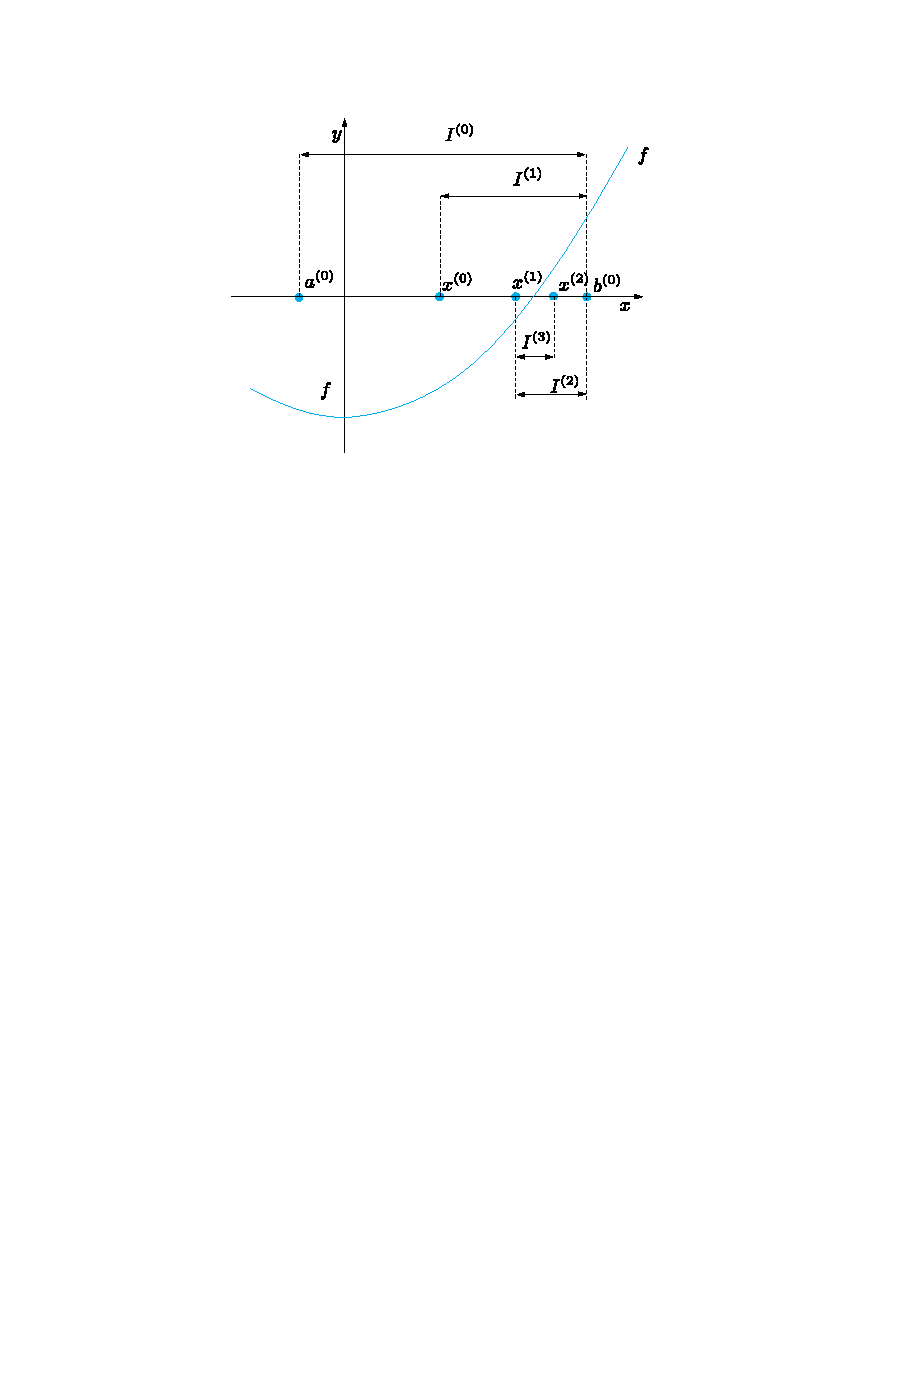
\includegraphics[width=.7\textwidth]{img/metodo-di-bisezione-1.pdf}
            \captionof*{figure}{Iterazioni effettuate.\cite{quarteroni2017calcolo}}
        \end{center}
        
        \noindent
        Si noti che ogni intervallo $I^{(k)}$ contiene lo zero $\alpha$. Inoltre, la successione $\left\{x^{(k)}\right\}$ converge necessariamente allo zero $\alpha$ in quanto ad ogni passo l'ampiezza $\left| I^{(k)} \right| = b^{(k)} - a^{(k)}$ dell'intervallo $I^{(k)}$ si dimezza.
    \end{examplebox}

    \noindent
    Il valore $I^{(k)}$ può essere riassunto come:
    \begin{equation*}
        \left|I^{(k)}\right| = \left(\dfrac{1}{2}\right)^{k} \cdot \left| I^{(0)} \right|
    \end{equation*}
    E di conseguenza l'\textbf{errore al passo} $\bm{k}$ può essere calcolato come:
    \begin{equation*}
        \left| e^{(k)} \right| = \left| x^{(k)} - \alpha \right| < \dfrac{1}{2} \cdot \left| I^{(k)} \right| = \left(\dfrac{1}{2}\right)^{k+1} \cdot \left(b-a\right)
    \end{equation*}
    Inoltre, data una certa \textbf{tolleranza} $\varepsilon$, per \textbf{garantire che l'errore al passo $k$ sia minore della tolleranza data} (ovvero, $\left| e^{(k)} \right| < \varepsilon$), basta applicare la seguente formula:
    \begin{equation}
        k_{\min} > \log_{2} \left(\dfrac{b-a}{\varepsilon}\right) - 1
    \end{equation}
    Dove $k_{\min}$ rappresenta il \textbf{numero \underline{minimo} di iterazioni prima di trovare un intero che soddisfi la disuguaglianza}.

    \begin{flushleft}
        \textcolor{Red2}{\faIcon{exclamation-triangle} \textbf{Possibile svantaggio}}
    \end{flushleft}
    Il metodo di bisezione \textbf{non garantisce una riduzione monotona dell'errore}, ma solo il dimezzamento dell'ampiezza dell'intervallo all'interno del quale si cerca lo zero. Infatti, \textbf{non viene tenuto conto del reale andamento di} $f$ e questo può provocare il mancato coinvolgimento di approssimazioni di $\alpha$ accurate.

    \newpage

    \subsection{Il metodo di Newton}

    Il \definition{metodo di Newton} sfrutta la funzione $f$ maggiormente rispetto al metodo di bisezione, usando i suoi valori e la sua derivata.

    \highspace
    Si ricorda che la retta tangente alla curva $\left(x, f\left(x\right)\right)$ nel punto $x^{(k)}$ è:
    \begin{equation*}
        y\left(x\right) = f\left(x^{(k)}\right) + f'\left(x^{(k)}\right)\left(x-x^{(k)}\right)
    \end{equation*}
    \textbf{Cercando} un $x^{\left(k+1\right)}$ tale che la \textbf{retta tangente in quel punto sia uguale a zero} $y\left(x^{\left(k+1\right)}\right) = 0$, allora si trova:
    \begin{equation}\label{eq: metodo di Newton}
        x^{\left(k+1\right)} = x^{\left(k\right)} - \dfrac{f\left(x^{\left(k\right)}\right)}{f'\left(x^{\left(k\right)}\right)} \hspace{2em} k \ge 0
    \end{equation}
    Purché la derivata prima nel punto $x^{(k)}$ sia diversa da zero, cioè $f'\left(x^{k}\right) \ne 0$.

    \highspace
    Questa equazione consente di calcolare una successione di valori $x^{(k)}$ a partire da un dato iniziale $x^{(0)}$. In altre parole, il \textbf{metodo di Newton calcola lo zero di $f$ sostituendo localmente a $f$ la sua retta tangente}.

    \highspace
    A differenza del metodo di bisezione, tale \textbf{metodo converge allo zero in un solo passo quando la funzione $f$ è lineare}, ovvero nella forma $f\left(x\right) = a_{1}x + a_{0}$.

    \begin{flushleft}
        \textcolor{Red2}{\faIcon{exclamation-triangle} \textbf{Limitazione}}
    \end{flushleft}
    La \textbf{convergenza} del metodo di Newton \underline{non} è garantita \textbf{per ogni scelta} di $x^{(0)}$, ma \textbf{soltanto} per valori di $x^{(0)}$ \textbf{sufficientemente vicini} ad $\alpha$, ovvero \textbf{appartenenti ad un intorno} $I\left(\alpha\right)$ sufficientemente piccolo di $\alpha$.

    \highspace
    Alcune osservazioni a seguito anche di questa limitazione:
    \begin{itemize}
        \item A seguito di questa limitazione, risulta evidente che se $x^{(0)}$ è stato scelto opportunamente e se lo zero $\alpha$ è semplice ($f'\left(\alpha\right) \ne 0$), allora il metodo converge.
        
        \item Nel caso in cui $f$ è derivabile con continuità pari a due, allora si ottiene la seguente convergenza:
        \begin{equation}
            \displaystyle \lim_{k \rightarrow \infty} \dfrac{x^{\left(k+1\right) - \alpha}}{\left(x^{(k)} - \alpha\right)^{2}} = \dfrac{f''\left(\alpha\right)}{2f'\left(\alpha\right)}
        \end{equation}
        Il significato è: se $f'\left(\alpha\right) \ne 0$ il metodo di Newton converge almeno quadraticamente o con ordine 2.

        In parole povere, \textbf{per $k$ sufficientemente grande, l'errore al passo $\left(k+1\right)$-esimo si comporta come il quadrato dell'errore al passo $k$-esimo, moltiplicato per una costante indipendente da $k$}.

        \item Se lo zero $\alpha$ ha molteplicità $m$ maggiore di $1$, ovverosia:
        \begin{equation*}
            f'\left(\alpha\right) = 0, \dots, f^{\left(m-1\right)}\left(\alpha\right) = 0
        \end{equation*}
        Allora il metodo di Newton è ancora convergente, purché $x^{(0)}$ sia scelto opportunamente e $f'\left(x\right) \ne 0$ $\forall x \in I\left(\alpha\right) \setminus \left\{\alpha\right\}$. Tuttavia in questo caso l'ordine di convergenza è pari a 1. In tal caso, l'ordine 2 può essere ancora recuperato usando la seguente relazione al posto dell'equazione~\ref{eq: metodo di Newton} ufficiale:
        \begin{equation}
            x^{\left(k+1\right)} = x^{(k)} - m \cdot \dfrac{f\left(x^{(k)}\right)}{f'\left(x^{(k)}\right)} \hspace{2em} k \ge 0
        \end{equation}
        Purché $f'\left(x^{(k)}\right) \ne 0$. Naturalmente, questo \textbf{metodo di Newton modificato} richiede una conoscenza a priori di $m$.
    \end{itemize}

    \longline

    \subsubsection{Come arrestare il metodo di Newton}

    Data una tolleranza fissa $\varepsilon$, esistono due tecniche applicabili per capire quando è necessario fermarsi ed evitare di continuare ad iterare:
    \begin{itemize}
        \item La \definition{differenza fra due iterate consecutive}, il quale si arresta in corrispondenza del più piccolo intero $k_{\min}$ per il quale:
        \begin{equation}
            \left| x^{\left(k_{\min}\right)} - x^{\left(k_{\min} - 1\right)} \right| < \varepsilon
        \end{equation}
        (test sull'incremento).

        \item Un'altra tecnica applicata anche per altri metodi iterativi è il \definition{residuo} al passo $k$, il quale è definito come:
        \begin{equation*}
            r^{(k)} = f\left(x^{(k)}\right)
        \end{equation*}
        Che è nullo quando $x^{(k)}$ è uno zero di $f$. In questo modo, il metodo viene arrestato alla prima iterata $k_{\min}$:
        \begin{equation}
            \left| r^{\left(k_{\min}\right)} \right| = \left| f\left(x^{\left(k_{\min}\right)}\right) \right| < \varepsilon
        \end{equation}
        Da notare che tale tecnica fornisce una \textbf{stima accurata dell'errore} \underline{solo quando} $\left| f'\left(x\right) \right|$ è circa pari a $1$ in un intorno di $I_{\alpha}$ dello zero $\alpha$ cercato.

        \underline{\textbf{Attenzione!}} Se la derivata non è circa pari a $1$ in un intorno dello zero cercato, la tecnica porterà:
        \begin{itemize}
            \item Ad una \textbf{sovrastima} dell'errore se $\left| f'\left(x\right) \right| \gg 1$ per $x \in I_{\alpha}$
            \item Ad una \textbf{sottostima} dell'errore se $\left| f'\left(x\right) \right| \ll 1$ per $x \in I_{\alpha}$
        \end{itemize}
    \end{itemize}

    \newpage

    \subsection{Il metodo delle secanti}

    Nel caso in cui la funzione $f$ non sia nota, il metodo di Newton non può essere applicato. Per fortuna, arriva in soccorso il \definition{metodo delle secanti}, il quale esegue una valutazione di $f'\left(x^{(k)}\right)$ andando a sostituire quest'ultima con un \textbf{rapporto incrementale calcolato su valori di $f$ già noti}.

    \highspace
    Più formalmente, assegnati due punti $x^{(0)}$ e $x^{(1)}$, per $k \ge 1$ si calcola:
    \begin{equation}
        x^{(k+1)} = x^{(k)} - \left(\dfrac{f\left(x^{(k)}\right) - f\left(x^{(k-1)}\right)}{x^{(k)} - x^{(k-1)}}\right)^{-1} \cdot f\left(x^{(k)}\right)
    \end{equation}

    \begin{flushleft}
        \textcolor{Green3}{\faIcon{question-circle} \textbf{Quando converge?}}
    \end{flushleft}
    Il metodo delle secanti converge a seguito di certe condizioni:
    \begin{itemize}
        \item \textbf{Converge ad} $\bm{\alpha}$, se:
        \begin{itemize}
            \item $\alpha$ radice semplice\footnote{$f'\left(\alpha\right) \ne 0$};
            \item $I\left(\alpha\right)$ è un opportuno intorno di $\alpha$;
            \item $x^{(0)}$ e $x^{(1)}$ sono sufficientemente vicini ad $\alpha$
            \item $f'\left(x\right) \ne 0$ $\forall x \in I\left(\alpha\right) \setminus \left\{\alpha\right\}$
        \end{itemize}

        \item \textbf{Converge con ordine} \definition{$p$ super-lineare}, se:
        \begin{itemize}
            \item $f \in \mathcal{C}^{2}\left(I\left(\alpha\right)\right)$
            \item $f'\left(\alpha\right) \ne 0$
        \end{itemize}
        Ovvero, esiste una costante $c > 0$ tale che:
        \begin{equation}
            \left| x^{\left(k+1\right)} - \alpha\right| \le c\left| x^{(k)} - \alpha \right|^{p} \hspace{2em} p = \dfrac{1 + \sqrt{5}}{2} \approx 1.618\dots
        \end{equation}

        \item \textbf{Convergenza lineare}, se:
        \begin{itemize}
            \item Radice $\alpha$ è multipla.
        \end{itemize}
        Come succederebbe usando il metodo di Newton.
    \end{itemize}

    % TODO: pag. 59

    \newpage

    \bibliography{bibtex}{}
    \bibliographystyle{plain}

    \newpage

    \printindex
\end{document}